%% ============================================================================
%% fig_2_4_retention_branch_detail.tex -- TikZ source of thesis Figure 10 (label
%% fig:retention_variants, Ch.2 Section "Retention Branch"). Drawn with the styles of
%% the architecture figure of the companion journal paper, in the notation of the
%% thesis. Every element follows the thesis text and the v20 code (cells 6, 21, 23, 25
%% of 04-final-v20/CLAM_TR_v20_UNI_Colab.ipynb):
%%   - 8 heads per module, head dimension 64, Q/K/V Linear 512 -> 64 without bias,
%%     s = 1/sqrt(64); one head type per configuration;
%%   - (a) RetNet: softmax(s QK^T) V, no decay, no coordinates;
%%   - (b) SpatialMult, SpatialMultRetNet: softmax(s QK^T (.) D^(h)) V;
%%   - (c) SpatialAdd: softmax(s QK^T + log(D^(h) + eps)) V;
%%   - D^(h)_ij = gamma_h^(||c_i - c_j|| / d_max), d_max over the K selected patches
%%     (+ eps); gamma_h fixed per head (gamma bank), never learned;
%%   - concat + output projection Linear 512 -> 512 (all four modules), then for RetNet
%%     and SpatialMultRetNet only: Dropout -> GroupNorm(8) -> + H_I -> SwishGate ->
%%     FFNBlock (pre-LayerNorm, 512 -> 2048 GELU -> 512, residual);
%%   - M_ret = mean over the K selected patches; DualBranch: no module.
%%
%% Sizes (KTU thesis guide, section 5.1: figure text >= 10 pt), laid out for 10 pt
%% text at scale 1: \footnotesize = 10.5 pt (titles, formulas), \scriptsize =
%% 10.05 pt (details, arrow labels); math sub/superscripts 7.04 pt (the script size
%% of 10 pt text, the guide's exception).
%% The fraction 1/K uses \dfrac so that 1 and K print at text size.
%% Layout: inputs; heads container (header and decay box, then panels (a)-(c));
%% the output projection below the container; the enhancement block (d) as a full-
%% width row below it; mean and fusion at the bottom.
%% Natural width < \textwidth (15.5 cm): include with width=\textwidth (scale ~1).
%% ============================================================================
\documentclass[border=1pt]{standalone}
\usepackage[T1]{fontenc}
\usepackage{amsmath}
\usepackage{newtxtext,newtxmath}
\usepackage{tikz}
\usetikzlibrary{arrows.meta,calc,positioning,fit,backgrounds}

%% ---- every non-script text item >= 10 pt at printed size ---------------------------------------------------
\makeatletter
\renewcommand\footnotesize{\@setfontsize\footnotesize{10.5}{12.6}}
\renewcommand\scriptsize{\@setfontsize\scriptsize{10.05}{12.1}}
\makeatother
\DeclareMathSizes{10}{10}{7.04}{7.04}
\DeclareMathSizes{10.05}{10.05}{7.04}{7.04}
\DeclareMathSizes{10.5}{10.5}{7.35}{7.04}
\hyphenpenalty=10000
\exhyphenpenalty=10000
%% -------------------------------------------------------------------------------------------------------------
\begin{document}
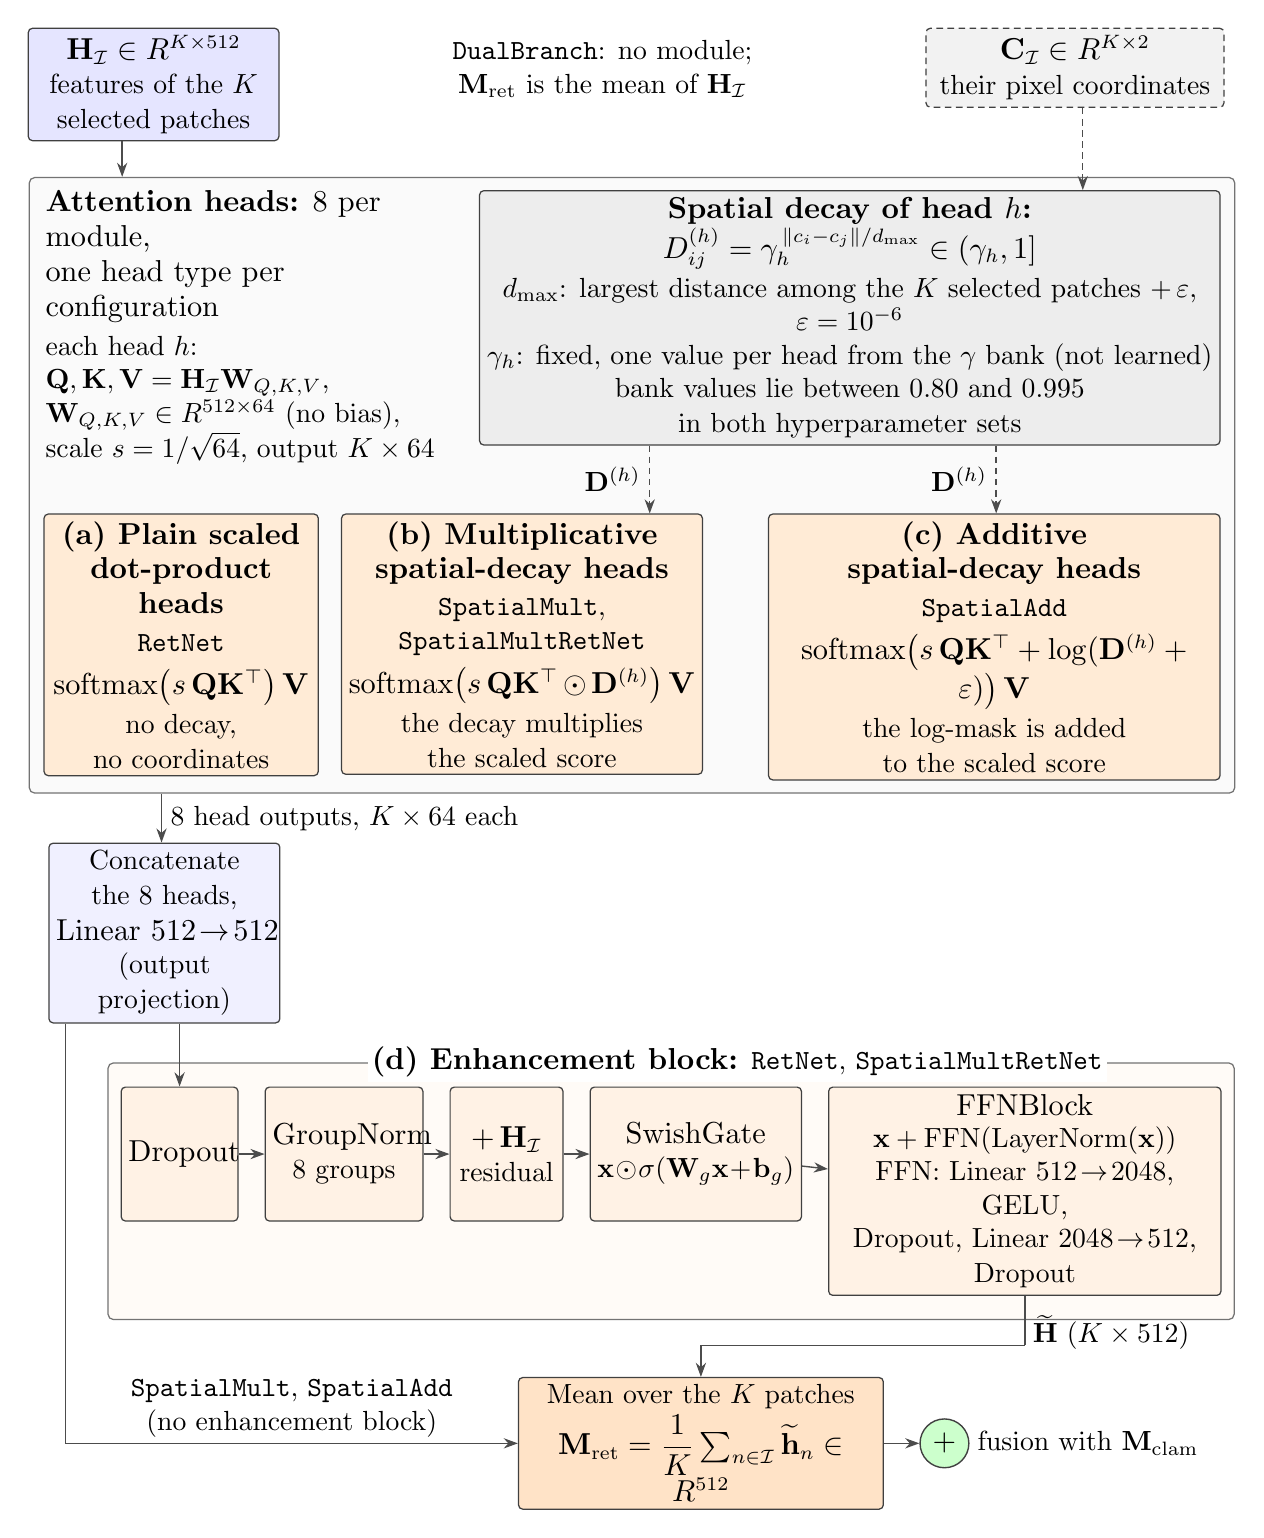
\begin{tikzpicture}[
  font=\footnotesize,
  >={Stealth[length=1.8mm,width=1.3mm]},
  base/.style={draw=black!75, rounded corners=1.5pt, line width=0.45pt,
               align=flush center, inner sep=2.6pt},
  chip/.style={base, fill=blue!10, minimum height=6mm},
  dchip/.style={chip, dash pattern=on 2.4pt off 1.6pt, fill=black!5},
  panel/.style={base, fill=orange!16, minimum height=26mm},
  decay/.style={base, fill=black!7},
  proj/.style={base, fill=blue!6, minimum height=15mm},
  enh/.style={base, fill=orange!10, minimum height=17mm},
  meanbox/.style={base, fill=orange!22, minimum height=12mm},
  sm/.style={draw=black!75, circle, minimum size=6.2mm, inner sep=0pt, fill=green!20,
             line width=0.5pt, font=\footnotesize},
  ar/.style={->, line width=0.5pt, draw=black!70},
  dar/.style={->, line width=0.5pt, draw=black!70, dash pattern=on 2.4pt off 1.6pt},
  lab/.style={font=\scriptsize, inner sep=1pt},
  legend/.style={font=\footnotesize, fill=white, inner sep=1.5pt}
]

% ---------------------------- inputs -----------------------------------------
\node[chip, anchor=north west, text width=3.00cm] (hin) at (0,0)
  {$\mathbf{H}_{\mathcal{I}}\in\mathbb{R}^{K\times512}$\\ {\scriptsize features of the $K$\\ selected patches}};
\node[dchip, anchor=north east, text width=3.60cm] (cin) at (15.20,0)
  {$\mathbf{C}_{\mathcal{I}}\in\mathbb{R}^{K\times2}$\\ {\scriptsize their pixel coordinates}};
\node[lab, anchor=north, align=center] at ($(hin.north east)!0.5!(cin.north west)+(0,-0.12)$)
  {\texttt{DualBranch}: no module;\\ $\mathbf{M}_{\mathrm{ret}}$ is the mean of $\mathbf{H}_{\mathcal{I}}$};

% ---------------------------- heads container contents -----------------------
\path (hin.south) ++(0,-0.62) coordinate (ytop);
\node[anchor=north west, text width=5.30cm, align=flush left, inner sep=0pt] (hdr) at (0.22,0 |- ytop)
  {\textbf{Attention heads:} 8 per module,\\ one head type per configuration\\[2pt]
   {\scriptsize each head $h$: $\mathbf{Q},\mathbf{K},\mathbf{V}=\mathbf{H}_{\mathcal{I}}\mathbf{W}_{Q,K,V}$,\\
    $\mathbf{W}_{Q,K,V}\in\mathbb{R}^{512\times64}$ (no bias),\\
    scale $s=1/\sqrt{64}$, output $K\times64$}};
\node[decay, anchor=north east, text width=9.22cm] (dec) at (15.15,0 |- ytop)
  {\textbf{Spatial decay of head $h$:} \
   $D^{(h)}_{ij}=\gamma_{h}^{\,\lVert c_{i}-c_{j}\rVert/d_{\max}}\in(\gamma_{h},1]$\\[2pt]
   {\scriptsize $d_{\max}$: largest distance among the $K$ selected patches $+\,\varepsilon$,\\ $\varepsilon=10^{-6}$\\
    $\gamma_{h}$: fixed, one value per head from the $\gamma$ bank (not learned)\\
    bank values lie between 0.80 and 0.995\\ in both hyperparameter sets}};

% panels start below the lower of the header and the decay box
\path let \p1=(hdr.south), \p2=(dec.south) in coordinate (yp) at (0,{min(\y1,\y2)-0.62cm});
\node[panel, anchor=north west, text width=3.30cm] (pa) at (0.20,0 |- yp)
  {\textbf{(a) Plain scaled\\ dot-product heads}\\[1pt]
   {\scriptsize\texttt{RetNet}}\\[3pt]
   $\operatorname{softmax}\bigl(s\,\mathbf{Q}\mathbf{K}^{\top}\bigr)\,\mathbf{V}$\\[2pt]
   {\scriptsize no decay,\\ no coordinates}};
\node[panel, anchor=north west, text width=4.40cm] (pb) at ($(pa.north east)+(0.28,0)$)
  {\textbf{(b) Multiplicative\\ spatial-decay heads}\\[1pt]
   {\scriptsize\texttt{SpatialMult},\\ \texttt{SpatialMultRetNet}}\\[3pt]
   $\operatorname{softmax}\bigl(s\,\mathbf{Q}\mathbf{K}^{\top}\odot\mathbf{D}^{(h)}\bigr)\,\mathbf{V}$\\[2pt]
   {\scriptsize the decay multiplies\\ the scaled score}};
\node[panel, anchor=north east, text width=5.55cm] (pc) at (15.15,0 |- yp)
  {\textbf{(c) Additive\\ spatial-decay heads}\\[1pt]
   {\scriptsize\texttt{SpatialAdd}}\\[3pt]
   $\operatorname{softmax}\bigl(s\,\mathbf{Q}\mathbf{K}^{\top}+\log(\mathbf{D}^{(h)}+\varepsilon)\bigr)\,\mathbf{V}$\\[2pt]
   {\scriptsize the log-mask is added\\ to the scaled score}};

\begin{scope}[on background layer]
  \node[draw=black!55, rounded corners=2pt, line width=0.45pt, fill=black!2,
        fit=(hdr)(dec)(pa)(pb)(pc), inner xsep=0.18cm, inner ysep=0.16cm] (cont) {};
\end{scope}

\draw[ar] (1.20,0 |- hin.south) -- (1.20,0 |- cont.north);
\draw[dar] (13.40,0 |- cin.south) -- (13.40,0 |- dec.north);
\draw[dar] (7.90,0 |- dec.south) -- (7.90,0 |- pb.north)
  node[lab, midway, left=2pt] {$\mathbf{D}^{(h)}$};
\draw[dar] (12.30,0 |- dec.south) -- (12.30,0 |- pc.north)
  node[lab, midway, left=2pt] {$\mathbf{D}^{(h)}$};

% ---------------------------- module tail -------------------------------------
\node[proj, anchor=north west, text width=2.75cm] (d1) at ($(cont.south west)+(0.25,-0.62)$)
  {{\scriptsize Concatenate\\ the 8 heads,}\\[0.5pt] \mbox{Linear $512\!\rightarrow\!512$}\\[-0.5pt]
   {\scriptsize (output projection)}};
\draw[ar] (1.70,0 |- cont.south) -- (1.70,0 |- d1.north)
  node[lab, midway, right=2pt] {8 head outputs, $K\times64$ each};

\path (d1.south) ++(0,-0.80) coordinate (ye);   % top of the chain boxes
\node[enh, anchor=north west, text width=1.30cm] (e1) at (1.18,0 |- ye) {Dropout};
\node[enh, anchor=north west, text width=1.82cm] (e2) at ($(e1.north east)+(0.33,0)$)
  {GroupNorm\\[-0.5pt] {\scriptsize 8 groups}};
\node[enh, anchor=north west, text width=1.25cm] (e3) at ($(e2.north east)+(0.33,0)$)
  {$+\,\mathbf{H}_{\mathcal{I}}$\\[-0.5pt] {\scriptsize residual}};
\node[enh, anchor=north west, text width=2.50cm] (e4) at ($(e3.north east)+(0.33,0)$)
  {SwishGate\\[-0.5pt] {\scriptsize $\mathbf{x}\odot\sigma(\mathbf{W}_{g}\mathbf{x}+\mathbf{b}_{g})$}};
\node[enh, anchor=north west, text width=4.80cm] (e5) at ($(e4.north east)+(0.33,0)$)
  {FFNBlock\\[-0.5pt]
   {\scriptsize $\mathbf{x}+\mathrm{FFN}(\mathrm{LayerNorm}(\mathbf{x}))$\\
    FFN: Linear $512\!\rightarrow\!2048$, GELU,\\ Dropout, Linear $2048\!\rightarrow\!512$,\\ Dropout}};
\draw[ar] (d1.south -| e1.north) -- (e1.north);
\foreach \u/\v in {e1/e2, e2/e3, e3/e4, e4/e5} \draw[ar] (\u) -- (\v);

\begin{scope}[on background layer]
  \node[draw=black!55, rounded corners=2pt, line width=0.45pt, fill=orange!3,
        fit=(e1)(e2)(e3)(e4)(e5), inner xsep=0.16cm, inner ysep=0.30cm] (dframe) {};
\end{scope}
\node[legend, anchor=west] at ($(dframe.north west)+(3.30,0)$)
  {\textbf{(d) Enhancement block:} {\scriptsize\texttt{RetNet}, \texttt{SpatialMultRetNet}}};

% ---------------------------- mean and fusion ---------------------------------
\path (dframe.south) ++(0,-0.72) coordinate (ym);
\node[meanbox, anchor=north, text width=4.45cm] (mean) at (8.55,0 |- ym)
  {{\scriptsize Mean over the $K$ patches}\\[1pt]
   $\mathbf{M}_{\mathrm{ret}}=\dfrac{1}{K}\sum_{n\in\mathcal{I}}\widetilde{\mathbf{h}}_{n}\in\mathbb{R}^{512}$};
\coordinate (elb) at ($(e5.south |- dframe.south)+(0,-0.32)$);
\draw[line width=0.5pt, draw=black!70] (e5.south) -- (elb);
\draw[ar] (elb) -| (mean.north);
\node[lab, anchor=west] at ($(e5.south |- dframe.south)+(0.06,-0.16)$)
  {$\widetilde{\mathbf{H}}$ ($K\times512$)};
\node[sm, anchor=west] (sum) at ($(mean.east)+(0.45,0)$) {$+$};
\draw[ar] (mean) -- (sum);
\node[lab, anchor=west] at ($(sum.east)+(0.06,0)$) {fusion with $\mathbf{M}_{\mathrm{clam}}$};

% bypass: modules without the enhancement block
\draw[ar] ($(d1.south west)+(0.22,0)$) |- (mean.west)
  node[lab, pos=0.75, above=1pt, align=center]
  {\texttt{SpatialMult}, \texttt{SpatialAdd}\\ (no enhancement block)};

\end{tikzpicture}
\end{document}
